\documentclass{css}
%\documentclass[english]{css}

\usepackage[dvipdfmx]{graphicx}
\usepackage{latexsym}
\usepackage{listings}
\usepackage{url}
\urlstyle{same}

\def\|{\verb|}

\newcommand{\cssyear}[0]{2025}
\newcommand{\cssname}[0]{CSS 2025}
\newcommand{\cssversion}[0]{2025/06/01}
\newcommand{\cssemail}[0]{css2025-office@iwsec.org}

\makeatletter
\newcommand\newblock{\hskip .11em\@plus.33em\@minus.07em}
\makeatother

\begin{document}

%% 本文が和文の場合,タイトル・著者名・著者所属・概要は,和文・英文共に必須.

\title{広範な脆弱性情報の統合管理と履歴追跡}
\etitle{Integrated Management and Historical Tracking of Diverse Vulnerability Information}

\affiliate{FUTURE}{フューチャー株式会社\\
Future Corporation}

%% メールアドレスは省略可能だが,代表者のメールアドレスは必須.
%% 姓名の間は半角スペースを入れること.

\author{中岡 典弘}{Norihiro Nakaoka}{FUTURE}[n.nakaoka.46@future.co.jp]
\author{篠原 俊一}{Shunichi Shinohara}{FUTURE}[s.shinohara.yx@future.co.jp]

\begin{abstract}
本研究は,脆弱性情報の収集・管理・提供における課題を解決するため,情報の履歴管理を中核とした新たな手法を提案する.
提案手法は,一次情報源からのデータ収集,共通データ構造への変換,およびデータベース構築の三段階からなり,各工程をバージョン管理システムと連携させることで,情報の追跡性・再現性・運用効率を大幅に向上させた.
実運用により,脆弱性情報の変更履歴を客観的事実として分析・共有できること,検知結果の完全な再現性が確保できること,ならびに運用安定性の向上を実証した.
今後はデータサイズの最適化や差分の意味的解析,パイプラインの堅牢化などを課題とし,より信頼性の高い脆弱性管理基盤の実現を目指す.
\end{abstract}

%% キーワード (1--5単語) の記載は任意.

\begin{jkeyword}
脆弱性情報,履歴管理,再現性
\end{jkeyword}

\begin{eabstract}
This study proposes a novel approach centered on history management to address challenges in vulnerability information collection, management, and provision.
The proposed method consists of three stages: data collection from primary sources, conversion to a common data structure, and database construction.
By integrating each stage with a version control system, the traceability, reproducibility, and operational efficiency of vulnerability information are significantly enhanced.
Through practical implementation, we demonstrated that changes in vulnerability information can be objectively analyzed and shared as factual records, complete reproducibility of detection results can be ensured, and operational stability is improved.
Future work will focus on optimizing data size, semantic analysis of differences, and hardening the pipeline to achieve a more reliable vulnerability management foundation.
\end{eabstract}

%% the following keyword part is optional and can be omitted.

\begin{ekeyword}
Vulnerability Information, History Management, Reproducibility
\end{ekeyword}

\maketitle

\section{はじめに}

我々は,オープンソース脆弱性スキャナであるVuls\cite{vuls}の開発を継続的に行っている.
本稿では,開発過程において直面した主な課題と,それに対する解決アプローチについて論じる.

第一の課題は,MITRE CVE\cite{mitre-cve}やNIST NVD\cite{nist-nvd}といった主要なデータソースにおいて,更新が遅延し,古い情報が長期間残存する場合がある点である.
このため,これらのデータソースを用いて脆弱性を検知した際に,未検知・誤検知が発生することがある.
例えば,CVE-2023-26207はFortinet FortiOSおよびFortiProxyに関する脆弱性である.
影響を受けるプロダクトとして,NIST NVDは図\ref{fig:cve-2023-26207-nvd}のように示しており,Fortinetでは図\ref{fig:cve-2023-26207-fortinet}のように示している.
Fortinetによると,FortiOS 7.0.0から7.0.15までのバージョンは影響を受けるとされているが,NIST NVDでは影響を受けるプロダクトとして示されていない.
つまり,NIST NVDの情報を信頼して脆弱性を検知した場合,未検知が発生する.
したがって,MITRE CVEやNIST NVDのみに依存せず,可能な限りベンダが直接公開するセキュリティアドバイザリなどの一次データソースから脆弱性情報を収集することが極めて重要である.

\begin{figure}[htbp]
    \begin{center}
            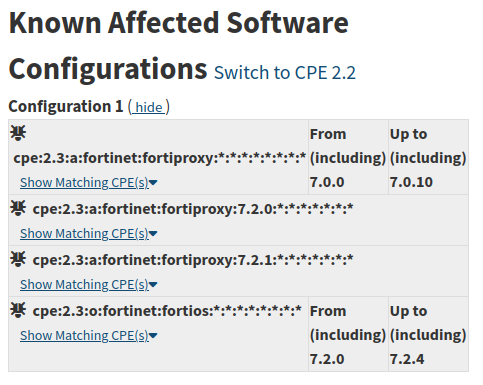
\includegraphics[scale=0.5]{./1-introduction/cve-2023-26207-nvd.png}
            \caption{NIST NVDによるCVE-2023-26207の影響を受けるプロダクト\cite{cve-2023-26207-nvd}}
            \label{fig:cve-2023-26207-nvd}
    \end{center}
\end{figure}

\begin{figure}[htbp]
    \begin{center}
        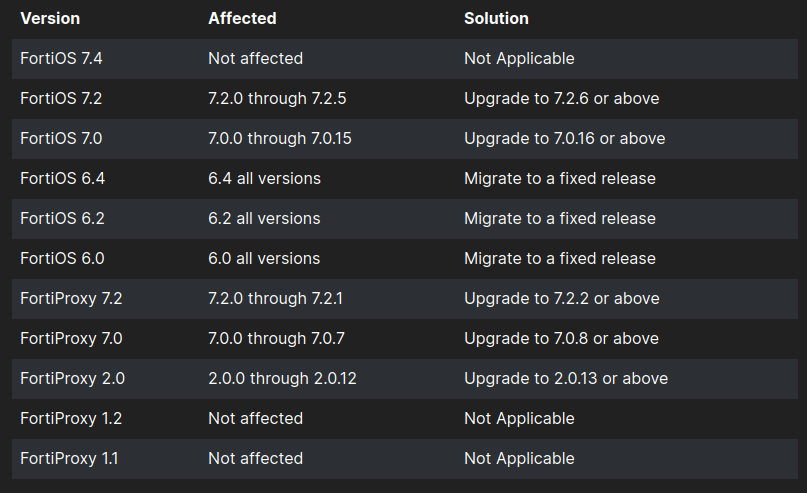
\includegraphics[scale=0.3]{./1-introduction/cve-2023-26207-fortinet.png}
        \caption{FortinetによるCVE-2023-26207の影響を受けるプロダクト\cite{cve-2023-26207-fortinet}}
        \label{fig:cve-2023-26207-fortinet}
    \end{center}
\end{figure}

第二の課題は,脆弱性情報が複数のデータフォーマットで提供されることである.
はじめに,開発者は提供されるそれぞれのフォーマットの仕様を理解することが求められる.
そして,実際に提供されるデータに沿って,さらにベンダ向けの調整が求められる.
例えば,2025年8月時点で,Red Hatは,OVAL形式\cite{redhat-ovalv2}とCSAF/VEX形式\cite{redhat-vex},OSV形式\cite{redhat-osv},CVE形式\cite{redhat-cve}の四つのフォーマットで脆弱性情報を提供している.
まず,開発者はこの4つのフォーマットを理解し,それぞれのフォーマットで記述された脆弱性情報の特徴を把握しなければならない.
OVAL形式は,メジャーバージョン毎に分かれ,未修正な脆弱性情報やExtended Update Supportの情報を含むかなどの観点で,さらに細かく分割されている.
対して,CSAF/VEX形式は,ID毎に提供されており,すべてのプロダクトに対する脆弱性情報が単一のファイルで提供される.
脆弱性と紐付けるパッケージの記述方法も異なる.
OVAL形式は,どのような脆弱性に対してもすべてバイナリパッケージ単位で紐付けるが,CSAF/VEX形式では,修正済みな脆弱性ではバイナリパッケージおよびソースパッケージの両方が紐付けされ,未修正や影響を受けない脆弱性においては,ソースパッケージ単位が紐付けされる\footnote{2025年8月時点で,CSAF/VEX形式において,未修正や影響を受けない脆弱性の場合でもバイナリパッケージ,ソースパッケージの両方を紐付けるように変更が進められている\cite{redhat-secdata-1097}.}.
このような違いにより,スキャナで収集する検知対象の情報や利用するデータフォーマットを適切に選択する必要が生じる.
Red Hatだけでなく,DebianやUbuntuなど多くのディストリビューションで,脆弱性情報が複数のフォーマットで提供されており,開発者にとって非常に負担となっている.
また,このデータフォーマットの違いは,利用者にも負担を与えており,脆弱性を検知するための必要な情報が検知対象毎に異なったり,誤検知を判断するとき,検知対象ごとに採用しているフォーマットと密接に結びついた実装を考慮する必要がある.

第三の課題は,脆弱性検知の再現性の確保や,検知結果の変化理由を説明することの困難さである.
従来は,ベンダから取得した脆弱性情報を直接変換し,脆弱性データベースを構築していた.
しかし,この方法では,例えばサーバーダウン等によりベンダから情報が取得できない場合,脆弱性データベースの更新が不可能となる.
また,誤検知の報告を受けた際,報告者が利用した脆弱性データベースを共有してもらわなければ,問題の再現や調査が困難であった.
さらに,検知結果に変化が生じた場合,たとえば以前検知されていた脆弱性が検知されなくなった場合,その理由を説明するためには,過去と現在の脆弱性データベースを比較する必要があるが,利用者が適切にデータベースを履歴管理していることは非常に稀である.

本研究では,これらの課題を解決するために以下の3点を達成する仕組みを提案し,評価する.
\begin{itemize}
    \item 一次データソースの情報をできる限り幅広く収集・採用することで,脆弱性情報の鮮度を保ち,未検知や誤検知のリスクを低減する.
    \item 収集した脆弱性情報を共通データ構造に変換することで,多くの開発者や利用者は脆弱性情報を一貫した形式で扱うことができ,異なるフォーマットの違いを意識する必要がなくなる.
    \item 収集したデータソースと共通データ構造に変換された脆弱性情報を履歴管理し、それらをもとに脆弱性データベースを構築することで,再現性や説明性,運用効率の向上を図る.
\end{itemize}
\section{提案手法}

本研究では,広範な脆弱性情報を効率的に収集し,利用者にとって扱いやすい形式へと変換・管理した上で,脆弱性データベースを構築し,提供する一連のプロセス「データハーベスト」を提案する.
本プロセスは,fetch・extract・db buildの3ステージから構成される.
図\ref{fig:data-harvest}は,各ステージの流れを示す.
fetchステージでは各ベンダーの脆弱性情報を入力とし,vuls-data-rawフォーマットのデータを出力する.
extractステージではvuls-data-rawフォーマットのデータを入力とし,共通スキーマに正規化されたvuls-data-extractedフォーマットのデータを出力する.
db buildステージではvuls-data-extractedフォーマットのデータを入力とし,脆弱性データベースを構築する.
また,データハーベストは継続的インテグレーション(Continuous Integration:CI)上で自動化されており,各ステージが効率的かつ安定的に運用される.
CIを用いた運用により,エラー発生時のパターン蓄積や,データ提供元の仕様変更・フォーマット変更への迅速な対応,障害発生時の復旧,信頼性の高い脆弱性情報の継続的な提供が可能となる.

\begin{figure*}[htbp]
  \begin{center}
    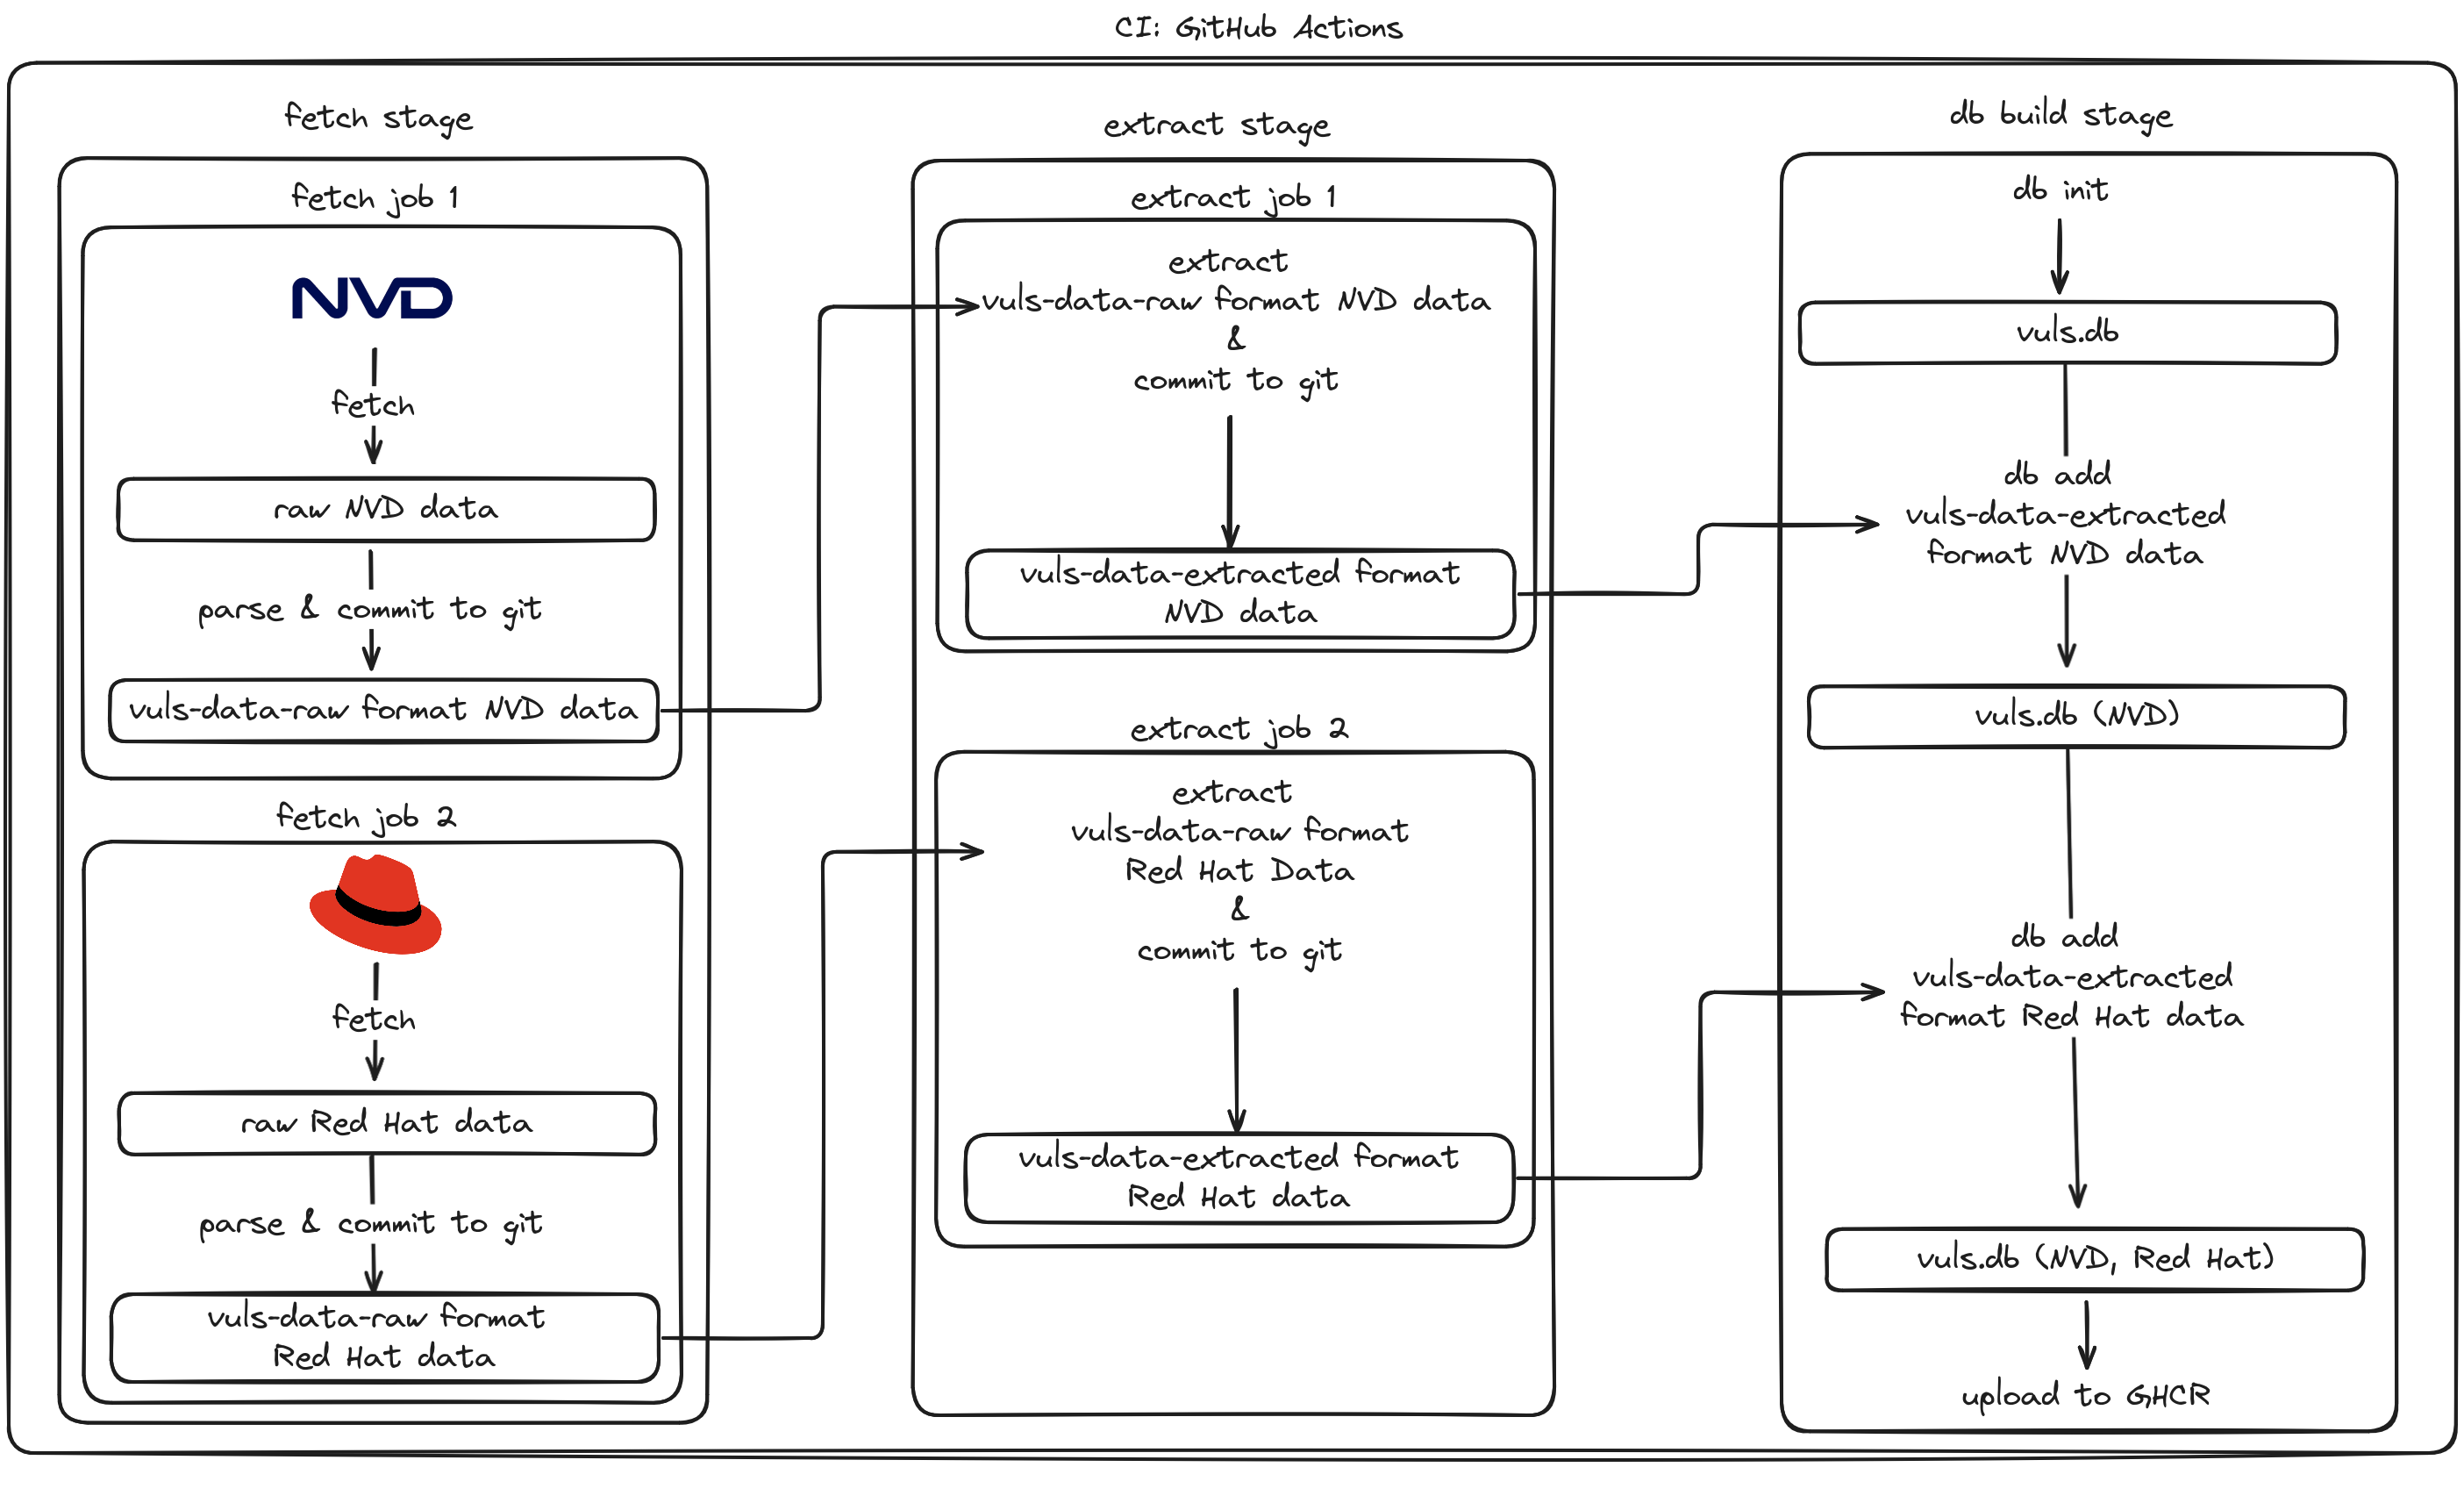
\includegraphics[scale=0.25,angle=90]{./2-methods/data-harvest.png}
    \caption{データハーベスト}
    \label{fig:data-harvest}
  \end{center}
\end{figure*}


\subsection{fetch ステージ(データ収集)}
fetchステージでは,一次データソースから脆弱性情報を収集する.
元のデータの構造をできるだけ保持しつつ,管理しやすい形に整形した状態をvuls-data-rawフォーマットと呼ぶ.
また,保存・管理にはバージョン管理システム(Git)を採用する.
Gitを用いることで,一次データソースの提供元がサーバーダウンして,収集に失敗したとしても,過去に成功した時点のデータを利用できたり,データの差分抽出や履歴管理が容易となり,データの更新や修正の追跡が効率的に行える.

\subsection{extract ステージ(データ変換)}
extractステージでは,fetchステージで収集したvuls-data-rawフォーマットのデータを,共通なデータ構造であるvuls-data-extractedフォーマットへと変換する.
vuls-data-extractedは,vuls-data-rawフォーマットなデータを共通データ構造に正規化したものであり,これにより,多様なデータソースの「方言」を吸収する高度な抽象化レイヤーとして機能し,開発者を各仕様の複雑さから解放する.
extractステージも,fetchステージと同様に変換したデータをGitの管理下に置く.
これにより,vuls-data-rawフォーマットなデータが変更されたことによって,変換が一時的に失敗した場合でも,過去に成功した時点のデータを利用できるため,脆弱性データベースの構築プロセス全体が停止することを防ぐことができる.


\subsection{db build ステージ(データベース構築)}
db buildステージでは,vuls-data-extractedフォーマットのデータを,脆弱性スキャナや脆弱性調査で容易に活用できるような形式でデータベースに格納する.
構築された脆弱性データベースは,GitHub Container Registryを通じて配布され,広範な利用者への提供が実現される.

\section{評価}

第2章で述べた提案手法に基づき,脆弱性情報の収集および管理システムを実装した.本章では,実装したシステムを用いて,提案手法が広範な脆弱性情報を統合的に管理可能にし,また追跡可能性を向上させるかを評価し,その有効性を明らかにする.

\subsection{システム実装と成果物}

提案手法の設計に基づき,脆弱性情報の収集および管理システムを実装した.本システムの主要な成果物は以下の通りである.

\begin{itemize}
  \item データハーベストツール\footnote{\url{https://github.com/MaineK00n/vuls-data-update}}
  \item データベース構築ツール\footnote{\url{https://github.com/vulsio/vuls-data-db}}
  \item 収集および変換されたデータ(履歴付き)\footnote{\url{https://github.com/vulsio/vuls-data-db/pkgs/container/vuls-data-db}}
  \item 構築されたデータベース(履歴付き)\footnote{\url{https://github.com/vulsio/vuls-nightly-db/pkgs/container/vuls-nightly-db}}
\end{itemize}

本システムは,執筆時点において12時間ごとにデータ収集からデータベース構築までの一連のデータハーベスト処理を自動的に実行している.

\subsection{広範な脆弱性情報の収集}

fetch ステージは,可能な限り一次情報源からの脆弱性データ収集を実現した.具体的には,MITRE CVEやNIST NVDといった主要な脆弱性情報源に加え,OSディストリビューションベンダ(Microsoft,Red Hat,Ubuntuなど),ネットワークベンダ(Fortinet,Cisco,Palo Altoなど),およびプログラミング言語関連の脆弱性情報も網羅的に収集している.執筆時点での収集対象は141種類に上り,これにより広範な脆弱性情報を一元的に管理することが可能となった.

fetch ステージはCIジョブとして定義\footnote{\url{https://github.com/vulsio/vuls-data-db/blob/main/.github/workflows/fetch-all.yml}}されており.執筆時点では1日に2回起動しデータ収集を行う.

\subsection{統合されたデータフォーマットの実現}

収集される脆弱性データは,それぞれ異なるフォーマットで提供されている.例えば,OVALやCSAF/VEXのように規格化されたフォーマットであっても,その内部における情報の記述方法はベンダごとに多様であり,単にフォーマット規格に準拠しているだけでは,その解釈に一貫性を持たせることは困難である.

extractステージの実装により,これらの差異や解釈方法を吸収し,統合されたデータ形式\footnote{\url{https://github.com/MaineK00n/vuls-data-update/blob/nightly/pkg/extract/types/data/data.go}}への変換を実現した.このデータ形式のうち,脆弱性検知に用いられる主要な情報を以下に示す.

\begin{description}
  \item [エコシステム] \mbox{} \\
    検知対象の環境を表す.例として \texttt{redhat:9} や \texttt{ubuntu:24.04} などが挙げられる.
  \item [パッケージ] \mbox{} \\
    脆弱性が存在する単位を表す.ソースパッケージかバイナリパッケージかの区別,パッケージ名,またはCPE文字列などを含む.
  \item [影響を受けるバージョン範囲] \mbox{} \\
    脆弱性が存在するバージョン範囲.\texttt{less than},\texttt{equal} などの条件表現やそられの組み合わせを記述でき,バージョン範囲を柔軟に表現できる.バージョン文字列の解釈方法(e.g. セマンティックバージョニング,RPM 形式)も合わせて明示している.
\end{description}

このvuls-data-extractedフォーマットにより,元のデータで暗黙的に仮定されていたソースパッケージとバイナリパッケージの区別や,バージョン情報の解釈方法を事前に把握しておく必要がなくなり,明示された記述に従って情報を解釈するだけでよくなった.これにより,後続のデータベース構築や,そのデータベースを用いた脆弱性検知におけるフォーマット依存性が劇的に減少した.また,Red HatのOVALとCSAF/VEXのように,フォーマットが異なる脆弱性情報の比較も容易になっている.執筆時点では,24種類の情報源に対するvuls-data-extractedフォーマット化が完了している.

extract ステージもCIジョブとして定義\footnote{\url{https://github.com/vulsio/vuls-data-db/blob/main/.github/workflows/extract-all.yml}}されており,fetchステージに続いて実行される.

\subsection{履歴管理機能の実装と追跡可能性・再現性の向上}

本システムに実装された履歴管理機能は,脆弱性情報の追跡可能性と脆弱性検知結果の再現性という2つの側面から,脆弱性管理の質を大幅に向上させることが明らかになった.

\subsubsection{変更履歴の追跡による検知結果変動の原因分析}

本システムの第一の利点は,脆弱性情報の変更履歴を追跡し,それによって検知結果の変動原因を分析できる点にある.これにより,脆弱性情報がどのように変更されたかを可視化し,検知結果の変化に対する客観的な説明を可能にする.以下にRed Hat Enterprise Linux向けVEXフォーマットによる脆弱性情報の変化の具体例を示す.

この vuls-data-extracted フォーマットのデータは GitHub Container Repository \texttt{vuls-data-db}\footnote{\url{https://github.com/vulsio/vuls-data-db/pkgs/container/vuls-data-db}}にあり,タグ\texttt{vuls-data-extracted-redhat-vex-rhel}で取得できる\footnote{取得したバイナリを Zstandard で展開すると Gitの管理用ディレクトリ \texttt{.git/} だけが入った構造になっている.Git 操作で履歴取得やファイル閲覧が可能である.}.

\paragraph{OS パッケージに対するステータスの変化}
特定の脆弱性情報において,修正ステータスが「Out of support scope」から「Affected」へと変化する事例が確認された.具体的には,CVE-2024-0229 における \texttt{redhat:6} のOSパッケージ \texttt{tigervnc} に対する評価をみると,コミット \texttt{8c5e6158b4}(2025-07-10 15:03)では 「Out of support scope」であったが,その次のコミット\texttt{3e8d8d3bf5}(2025-07-11 05:07)で「Affected」へと変更されてたことが確認できた.

これは,サポート対象外とされていたパッケージが,後に影響を受けるものとして再分類されたことを意味する.本機能により,このようなステータスの変更がいつ,どのように発生したかを明確に把握できる.

\paragraph{特定のCVE IDに対する情報が消滅する事例}
ある時点で存在していた CVE-2024-24791 に関する情報が,その後の更新でシステムから消滅した事例が確認された.
具体的にはコミット \texttt{708ff21dc6}(2025-07-10 15:03:39)では CVE-2024-24791 のデータが存在する一方で,その次のコミット \texttt{e4787b5085}(2025-07-18 03:47)では該当 CVE データのファイルが存在しない.

この情報の削除の直接的な理由は不明であるが,データ提供者のポリシー変更やデータ生成時のエラーなど複数の可能性が考えられる.重要なのは,本方式がこのような「原因不明の変更」をも客観的な事実として捉え,その後の調査の起点とできる点にある.なお,Red Hatの VEX フォーマット以外の公式情報源である \cite{rh-cve-2024-24791-1} \cite{rh-cve-2024-24791-2} には,削除が確認された日 2025年7月18日 とその約1週間後の 2025年7月24日には情報が掲載されていたことを補足する.

\paragraph{Red Hat 10に対する情報のみが消滅する事例}
CVE-2024-43420に関する情報において,当初は\texttt{redhat:6},\texttt{redhat:8},\texttt{redhat:9}, \texttt{redhat:10}のエコシステムに対する検出情報が含まれていたが,その後の更新で\texttt{redhat:10}に関する情報のみが消滅した.具体的にはコミット \texttt{8c5e6158b4}(2025-07-10 15:03:39) では CVE-2024-43420 のデータに \texttt{redhat:10} が含まれていたが,その次のコミット \texttt{3e8d8d3bf5}(2025-07-11 05:07:05)では含まれなくなっていた.

このような特定のバージョンに対する情報の削除も,履歴管理機能によって明確に把握でき,影響範囲の特定や原因究明に役立つ.

以上のように,取得したタイミングに依存せず,明確なコミットハッシュという ID を示しつつ脆弱性データの変更点のトラッキングが可能になった.また,それはパブリックなインターネット上に公開されているため,誰でも変更について確認し,議論できる土台を提供する.

\subsubsection{特定時点における検知の再現性}

本システムの第二の利点は,特定の時点における脆弱性検知の再現性を可能にする点である.これは,脆弱性データベースを固定することで実現される.

従来,脆弱性情報を各自が任意のタイミングで取得していたため,「昨日の13時頃に取得したデータを使っている」といった曖昧な認識合わせしかできなかった.しかし,本方式では脆弱性データベースをそのハッシュ値で保存および参照することにより,検知結果の再現性を確実に保証できるようになった.検知ロジック自体はソースコードがGit管理されているため再現性が高いが,これに加えて脆弱性データ側の再現性を高めることができた点は極めて重要である.

例えば,バグ報告の issue \cite{issue-2198}では,確実な再現性のため \texttt{config.toml}設定ファイルのなかで脆弱性データベースのハッシュ値を明示的に指定している.こうすることで,以前は難しかった常に同じデータセットを用いた検知が可能となる.
データベースのハッシュ値が分かると,そのなかのメタデータに extracted と raw データの Git コミットハッシュが記されているため,一次情報源に近いところまで遡った調査も可能となる.

これは,バグ報告やセキュリティ監査など,特定の時点での状況を正確に再現する必要がある場合に,極めて強力な機能となる.

\subsection{エンジニアリング上の利点(補足)}

本方式は,上記の本質的な利点に加え,エンジニアリング面でもいくつかの恩恵をもたらした.

\begin{description}
  \item[脆弱性データ提供サーバへの依存性低減] \mbox{} \\
    脆弱性データをGitHub Container Registryに配置することで,各脆弱性データ提供サーバの状態(応答不能など)に直接依存することなく,データベースを生成できるようになった.これにより,DB生成時のエラー発生可能性が大幅に減少し,システムの堅牢性が向上した.
  \item[DB生成時間の安定化] \mbox{} \\
    上記の依存性低減と関連して,データベース生成にかかる時間が安定し,予測可能になった.これは運用上の大きなメリットとなる.
\end{description}

\section{考察}

本研究で提案した「データハーベスト」は,脆弱性情報の収集・統合・履歴管理を通じて,脆弱性管理のあり方に新たなパラダイムを提示する.本章では,その学術的および実務的な貢献を考察する.

本手法の核心は,脆弱性情報のある時点の情報だけでなく更新履歴までを管理対象とし、それをバージョン管理システムで体系的に管理するフレームワークを確立した点にある.これにより,従来は単一の時間に留まっていた脆弱性管理に対して「時間軸に沿った脆弱性情報の観測と分析」という観点を付加する.

このアプローチがもたらす最大の貢献は,脆弱性管理プロセスにおける説明責任と客観性の向上である.Gitによる履歴管理は,脆弱性情報のいかなる変更(例:ステータス変更や情報の追加・削除)も,共有可能な客観的事実として記録する.これにより,「なぜ検知結果が変わったのか」という問いに対し,従来のような推測ではなく,コミットハッシュと差分に基づいた明確な回答が可能になる.脆弱性データベースをハッシュ値で固定することによる検知結果の再現性保証は,プロセスの属人性を軽減し,過去の状況を正確に説明する上で不可欠な機能となる.

また,extractステージは,多様なデータソースの「方言」を吸収する高度な抽象化レイヤーとして機能し,開発者を各仕様の複雑さから解放する.我々が構築し公開するデータベースは,コミュニティがデータ収集という「車輪の再発明」を避けることを可能にし,オープンソースエコシステム全体の技術水準向上にも貢献する.

以上のことから,本手法は脆弱性情報の動的な性質を捉え,その管理に客観性,再現性,説明責任をもたらすことで,現代の脆弱性管理が直面する課題への有効な解決策となる.これは,日々の運用を効率化する実務的価値と,脆弱性情報を時間軸で管理するという新たな手法による学術的意義を併せ持つと結論づける.

\section{議論}

本章では,提案手法およびその実装について,実際の運用経験を踏まえた上で,将来の改善点と課題について議論する.

\subsection{データサイズの最適化}
現状のシステムでは,広範な脆弱性情報を継続的に収集し履歴管理を行っているが,ベンダーやフォーマットによっては元の脆弱性情報がギガバイトを超えるサイズになる場合がある.これを履歴管理すると,データサイズはさらに増大する.現在のクラウドベースのシステムやストレージにおいては,ギガバイトオーダーのデータを保持すること自体は難易度が低いものの,脆弱性検知のためにこれらのデータを効率的に配布し,継続的に更新し続けるためには,データサイズをできるだけ小さく保つことが望ましい.

データサイズを削減するための候補となる手段を以下に示す.

\subsubsection{シリアライズフォーマットの改善}

現状はJSONをシリアライズフォーマットとして非構造化データに近い形で保持しているが,よりサイズ効率の高いフォーマットへの移行が考えられる.

\begin{description}
  \item[スキーマ情報を利用したシリアライズ] \mbox{} \\
    例えば,Protocol Buffersのようなスキーマベースのシリアライズ形式を用いることで,JSONよりも小さいサイズでデータを保持することが可能である.これにより,ネットワーク転送量やストレージ使用量を削減できる.
  \item[より構造化データに近い形でのシリアライズ] \mbox{} \\
    カラム型データストア(e.g. Parquet\cite{parquet})にデータを格納することで,大幅な圧縮効果が期待できる.ただし,脆弱性情報には再帰構造が含まれるため,その構造化とアクセス方法について慎重な設計が必要となる.これが実現できれば,カラム型ストアの特性を活かした高い圧縮率と効率的なデータアクセスが期待できる.
\end{description}

\subsubsection{データベース内部での圧縮}
現状,脆弱性データベースはJSONがそのまま格納されたBoltDB形式をZstandardで圧縮して配布し,利用時に展開してストレージに配置している.DB内部に圧縮機能を持ったエンジンを利用することで,配布時と利用時の両方でサイズを削減できる可能性がある.候補の例としては,SQLite3のプラグインで圧縮機能を提供するもの(e.g. sqlite-zstd\cite{sqlite-zstd})や,LSM-treeベースのデータベースにおけるブロック単位の圧縮機能(e.g. RocksDB\cite{rocksdb}, Pebble\cite{pebble})が挙げられる.これらの技術を導入することで,ストレージ効率と配布効率のさらなる向上が期待される.

\subsection{差分の論理的な説明能力の向上}
現在,履歴管理は実現されているものの,時系列差分の確認方法はJSON文字列の簡易な行ベースの差分に限定されている.このような差分には,更新日付のみの変更のような軽微なものから,未修正だった脆弱性があるバージョンで修正されたといった利用者にとって極めて重要な情報まで,様々な種類の変更が混在している.

脆弱性に関して重要な変更点を,人間に分かりやすい形で表現できるようになれば,脆弱性への対応にかかる人的負荷を大幅に軽減できる.そのためには,JSON文字列としてではなく,構造化されたデータとして差分を抽出・解析できる機能が望ましい.これにより,以下のような機能を提供できるようになるだろう.
\begin{description}
  \item[重要履歴の抽出] \mbox{} \\
    ある期間で多くの変更点が入っている場合でも,利用者にとって特に重要な差分がある履歴だけを効率的に抽出する機能.
  \item[論理的な差分提示] \mbox{} \\
    単純な行ベース差分ではなく,脆弱性のステータス変更,影響範囲の更新,修正バージョンの追加など,より論理的な構造として差分を提示する機能.
\end{description}

これらの機能は,利用者が脆弱性情報の変化を迅速に理解し,適切な対応を決定する上で大きな助けとなる.

\subsection{データ生成パイプライン(CI)の安定性}
ベンダの脆弱性情報を取得する部分において,相手サーバーの応答遅延や,全く応答しないといったエラーが発生することがあり,これがデータの更新間隔の長期化を招くことがある.また,相手先サーバー側の仕様変更などによって取得プログラムがエラーとなり,プログラムが修正されるまでしばらく更新が停止することも起こり得る.

本システムのデータ生成パイプラインであるCIのさらなる安定化は重要な課題である.これには,リトライ機構の強化,エラー発生時の自動通知と復旧プロセスの改善,そしてベンダー側のAPI変更に対する柔軟な対応メカニズムの導入などが含まれる.パイプラインの安定性は,提供される脆弱性情報の鮮度と信頼性を直接的に左右するため,継続的な改善が必要である.


\bibliographystyle{junsrt}
\bibliography{./1-introduction/intro.bib,./3-evaluation/evaluation.bib,./5-conclusion/conclusion.bib}

\end{document}
